\documentclass{article}
\usepackage[utf8]{inputenc}
\usepackage{graphicx}
\title{COP290\\Assignment 3}
\author{Harishchandra Patidar\and Rohit\and Sachin Kumar\and Manoj Kataria}

\begin{document}

\maketitle
\begin{center}
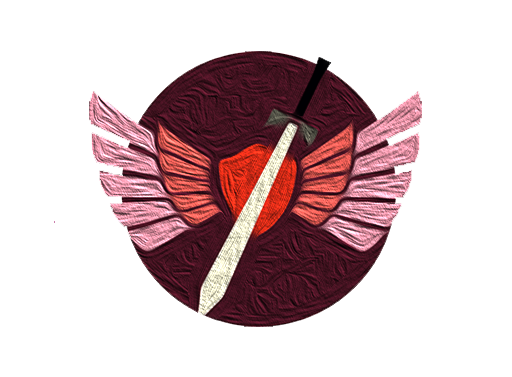
\includegraphics[height=4cm]{icon.png}\\
\textbf{Battle and Chaos}
\end{center}
\newpage
\tableofcontents
\newpage

\section{Introduction}

In this assignment, we will be building a multi-player game \textbf{Battle and Chaos}. Many variations of this type of game are available but none of them have the multi-player feature. This game is sort of mixture of real time strategy, action and tower defence.

\section{Game Description}
There will be two teams in the game. Each team will have equal number of players (bots if required).\\\\
Each team will have
\begin{itemize}
\item \textbf{Base} which it has to defend. The team which destroys the opponent team's base will be victorious.
\item \textbf{Attacking units} to destroy opposition's base. The team can release attacking units(if available) at any point of time.
\item \textbf{Defense units} to defend the base.
\end{itemize}
Our Game will have following basic units : 
\begin{itemize}
\item \textbf{Hero} :
Each player chooses a hero from a set of available heroes at the start of the game. A hero can move anywhere in the arena and its motion is controlled by player himself. It can attack enemy heroes and creeps. If a hero dies, it re-spawns after some time (or instantly if the player wish to spend some gold).

\item \textbf{Creeps} :
Creeps are the basic attacking units. Each team send creeps towards opponent teams base. Creeps move only on certain paths (there are many). The set of paths used by two teams is disjoint, therefore creeps of two teams do not collide with each other. The base is destroyed if a set amount of enemy units pass through it. Creeps are of various types and can be upgraded by the player.

\item \textbf{Towers} :
Towers are the basic defense units. Towers can be placed anywhere on the arena except in front of base or on the path on which enemy units move. Towers attack enemy units and heroes, by shooting bullets towards them, which adds some amount of gold to our bank depending upon initial health points of dead units. Towers are indestructible and of various types. Placing and upgrading towers costs gold.
\end{itemize}
Each team starts with some of these basic units and a fixed amount of gold. Each of the above units can be upgraded by spending gold. The cost of up-gradation increases as the units become more powerful.

\newpage
\section{Components}
The implementation of this game is broadly divided into the following components:
\begin{itemize}
\item Game Attributes
\item Graphics and Sounds
\item Networking
\item Artificial Intelligence
\end{itemize}

\section{Game Attributes}
Different units have different attributes. Description of general attributes of units:
\begin{itemize}
\item \textbf{Base} : has some initial HP(health points) which will decrease every time a creep passes through it or on attack by opposition heroes. The decrement will determined by following formula:\\\\
 $ HP_{f} = HP_{i} - HP_{Unit}*d$, where d is the decrement factor of unit 
\item \textbf{Tower} :
\begin{itemize}
\item range : in which it can shoot
\item damage : which it does to creeps
\item attack speed
\item cost
\item upgrade state : whether fully upgraded or can be upgraded further
\end{itemize}
\item \textbf{Creep} :
\begin{itemize}
\item movement speed
\item HP
\item cost
\item upgrade state
\end{itemize}
\item \textbf{Hero} :
\begin{itemize}
\item HP
\item damage : which it does to opposition heroes and their attacking units
\item attack speed
\item movement speed
\item range : in which it can attack
\item upgrade state
\end{itemize}
\end{itemize}
These attributes can be changed by spending gold.

\newpage
\section{Graphics and Sounds}
Overall, we will be implementing following things:
\begin{itemize}
\item Arena of the game
\item Different types of enemy units
\item Towers
\item Sound Effects
\item User Interaction using mouse
\end{itemize}
\subsection{Gameplay view}
The game will start with an arena in which there will be two bases one of each team, which they have to protect. The top view of the arena will be displayed.\\
\begin{center}
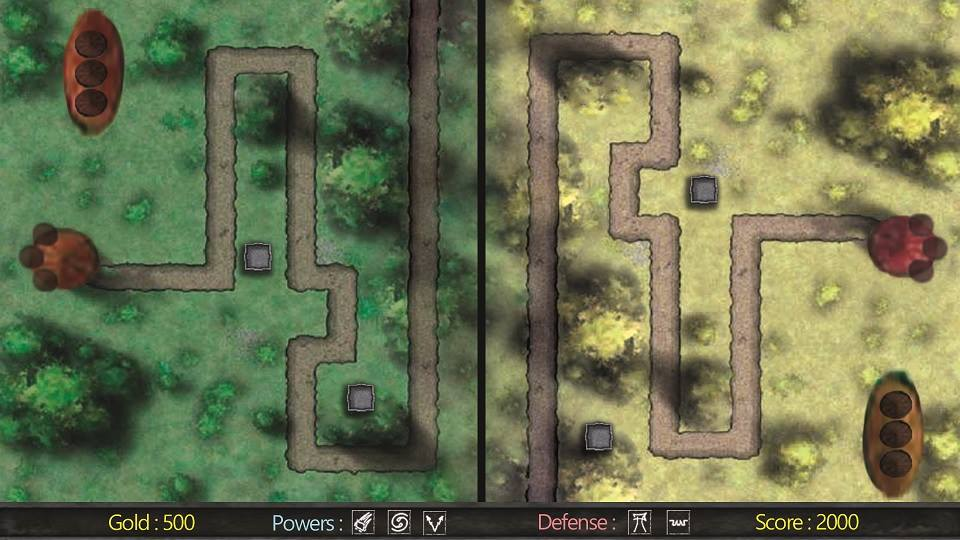
\includegraphics[width=11cm, height=8cm]{arena.png}
\end{center}
Now, to implement this we will be using SFML library for C++. We have to show towers, enemy units, base and make them interactive. User can click them and do some actions. Background will be a simple rectangle with an image texture mapped on it. Above it there will be another layer consisting of path.\\
Creeps and towers will be represented on the next layer.They will be rectangles, with alpha mapping and texture mapping. Alpha mapping will account for the custom shapes of the units.\\
\begin{center}

\includegraphics[width=1.5cm, height=1.5cm]{enemy.png}\hspace*{1cm}

\includegraphics[width=1.5cm, height=1.5cm]{towers.png}\hspace*{1cm}
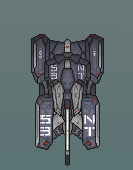
\includegraphics[width=2.5cm, height=2.5cm]{Hero.png}
\end{center}
Apart from the basic design, we need to make it look more beautiful, so there will be some texture mapping and more effects which are available in SFML library.
\subsection{Sound}
A mute game is no fun, so we will add sounds in the game. Sound effects will be very realistic with a fine background music to give the feel of the game. We will be using SFML library for sound. For playing small sounds we will use .wav files in sound buffer and for long music we will stream .ogg files in music buffer.
\subsection{Mouse Interaction}
Whenever a player clicks on the game screen,  using the co-ordinates of the clicked point we will calculate the unit which is being clicked and accordingly a menu for that unit will appear. The player can now choose one of the options from menu and change the attributes of selected unit.
\begin{center}
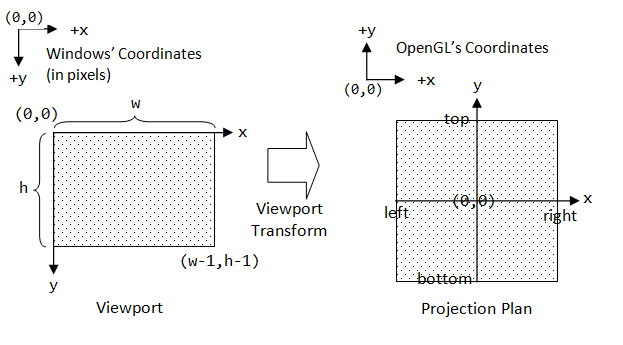
\includegraphics[height=7.0cm]{mouse.png}
\end{center}
\newpage
\section{Networking}
We describe here networking portion of game :
\begin{itemize}
\item The game will be server free.
\item It will be based on Peer-to-Peer network protocol.
\item One of the player starts the game and other player joins the game by connecting to all the other players.
\item The connection between two player will be established using TCP sockets.
\item Any person can leave the game during the game play.
\end{itemize}

\subsection{Connection}
We will be having following classes to implement networking in our game :
\begin{itemize}
\item class socket : open(),close(),send(),receive() methods
\item class connection : listen(),connect() methods
\end{itemize}
Since every player will be connected to all the other players, connections on one computer will be managed using threads for better synchronization between players.\\
If a player leaves the game mid-way or connection is lost then we will replace the player by a bot and game will remain balanced.

\subsection{Message Transfer}
Messages will be transferred when player,
\begin{itemize}
\item introduces new defense or attacking units.
\item upgrade/remove an existing unit.
\item changes direction of attacking units.
\item move its hero unit, basically these messages will be sent on every frame of the game since all the players should know that position of each other in sync.

\end{itemize}
Messages will be stored in two queues, one for the messages send by the player and one for the messages received. At each frame, each player will
\begin{itemize}
\item first process the incoming messages
\item send messages back to the network
\item render
\end{itemize}

\newpage
\section{Artificial Intelligence}
To make the game more interesting, we will require our basic units to have some intelligence in them. This will be a significant challenge.
\subsection{AI of basic units}
We describe here the AI component of each unit
\begin{itemize}
\item \textbf{Creeps} : As mentioned earlier, a wave of creeps will aim to reach opposition's base via a path which causes minimum damage to themselves. Creeps won’t always take the same route. To find the optimal path, we will use \textbf{Dijkstra's algorithm}. In the algorithm, the weight of an edge between two nodes(successive tiles of path) will be taken as damage that will be done to creep if it moves along that edge.\\
We will be using following formula to calculate weight of edge as:\\

$W \;= X*damage + 1 $\\
where X is a large constant. We need to minimize $\sum W $.\\

\item \textbf{Towers} : Towers will be shooting bullets on a wave of creeps in its range. In a wave, it will first shoot the creep which is closest to the base then try to shoot others if the first one is destroyed or goes out of range of tower.\\
This can be implemented using a simple data structure like queue. Whenever a creep comes in the range of the tower, it will be pushed into the queue of the tower and will be popped when the unit leaves the range of tower or destroyed. There will be some modification when the units are controlled freely by the player.
\end{itemize}
\subsection{AI of Bot}
Since the game will be a team game, so to have equal number of players on each side, we may require a bot. The bot will have to control its defense and attack units and deal with upgrading of powers. Following are the 3 components of AI of bot
\begin{itemize}
\item \textbf{Control Defense unit} : To defend its base, bot has to intelligently decide where to place towers. Also it has to decide which type of tower will cause maximal damage to opponent's enemy unit. So type of tower will be according to strength of opponent's attack unit.

\item \textbf{Control Attack unit} : Bot will be controlling creep's strength and size of creep unit to attack on opponent's base. It will be sending creeps after regular intervals of time. And it will decide the strength and number of creeps according to opponent's defense. To implement this, \textbf{FSM} will be used. Input to this FSM will be opponent's towers attributes and states will be strength and size of of creep unit. 

\item \textbf{Purchasing Items} : The Bot will earn gold coins after destroying creeps or heroes of opponent team. These gold coins will be used for purchasing and upgrading defense and attack units. The Bot will upgrade a tower/creep if it is more effective in neutralizing powers of opposition wave otherwise it will send waves or purchase new towers
\end{itemize}

\newpage
\section{Testing Components}
We describe here how will we debug each component :

\subsection{Graphics}
The graphics should work perfectly at good fps. So we will be testing the graphics separately first with large number of units in game and at high speed.
\subsection{Sound}
Background music is fine. But sound effects should be in sync with the game actions. We will need to test that mainly in the sounds part.
\subsection{Networking}
We will test networking part separately then integrate with the main program. To test we'll send continuous messages between computers on a test network. Latency should be as small as possible otherwise the game will not run properly.\\
All the bad cases (connection lost, low speed of network, etc.) should be handled, no crash/unwanted behaviour should occur.
\subsection{Artificial Intelligence}
To test Artificial Intelligence of each unit of game, we will try different permutations for testing both defensive and attacking units.\\
Defensive unit can be tested by sending enemy waves of different strength to opponent's side. \\
Attack unit's intelligence for path selection can be tested by placing different towers along path.
\end{document}
